%%%%%%%%%%%%%%%%%%%%%%%%%%%%%%%%%%%%%%%%%%
\section{Part 3 - Exercise 2 - slides 35-36}
%%%%%%%%%%%%%%%%%%%%%%%%%%%%%%%%%%%%%%%%%%
Consider the problem
\begin{align*}
	\min \left\{-\sum_{i=1}^m\log\left(\bs a_i^\top \bs x - b_i\right)+ \sum_{i=1}^{n-2} \sqrt{\left(x_i-x_{i+1}\right)^2+\left(x_{i+1}-x_{i+2}\right)^2}: a_i^\top \bs x > b_i, i\in [m] \right\}
\end{align*}
where $\bs a_i \in \mathbb{R}^n$ and $b_i \in \mathbb{R}$ for all $i\in [m]$. 

\indent (a) This problem matches the canonical problem 
\begin{align*}
	\min \left\{h_1(\bs x) + h_2(\bs v) \text{ s.t. }  \bs{Ax}+ \bs{Bv} = c \right\},
\end{align*}
with
\begin{itemize}
	\item $h_1(\bs x)=0$;
	\item $h_2(\bs v) = -\sum_{i=1}^m\log\left( v_i^{(1)} - b_i\right)+ \sum_{i=1}^{n-2} \sqrt{\left(v_i^{(2)}\right)^2+\left(v_i^{(3)}\right)^2}+ \delta_{\left\{\bs x|\bs x \geq \bs b\right\}}\left(v^{(4)}\right)$ with $\bs v = \begin{bmatrix}
		\bs v^{(1)} \\ \bs v^{(2)} \\ \bs v^{(3)} \\ \bs v^{(4)}
	\end{bmatrix}$;
	\item $\bs A = \begin{bmatrix}
		\Tilde{\bs  A} \\ \bs D \\ \bs E \\  \Tilde{\bs A} 
	\end{bmatrix}$, with $\Tilde{\bs A} = \begin{bmatrix}
		\bs a_1^\top \\ \vdots \\ \bs a_m^\top
	\end{bmatrix}$, $\bs D = \begin{bmatrix}
		1 & -1 &&& \\ 0 &1 &-1 && \\ && \ddots && \\ &&1&-1&0
	\end{bmatrix}$, $\bs E = \begin{bmatrix}
		0 &1 & -1 && \\ & &1 &-1 && \\ && \ddots && \\ &&&1&-1
	\end{bmatrix}$; $\bs B = -\bs I$; $\bs c = \bs 0$. 
\end{itemize}
In order to obtain the ADLPMM method, the proximal operators of $h_1$ and $h_2$ are needed. The first is obtained trivially as 
\begin{align*}
	\text{prox}_{\eta h_1}(\bs x) = \text{prox}_{0}(\bs x) = x. 
\end{align*}
For the second one, some preliminary computations are needed:
\begin{align*}
	\text{prox}_{- \eta \sum_{i=1}^m\log\left( v_i - b_i\right)}(\bs v) &= \text{prox}_{- \eta \sum_{i=1}^m\log\left( v_i \right)}(\bs v - \bs b) + \bs b,\\
	&= \frac{\bs v - \bs b+\sqrt{(\bs v - \bs b)^2+4\eta}}{2} + \bs b,\\
		&= \frac{\bs v + \bs b+\sqrt{(\bs v - \bs b)^2+4\eta}}{2},
\end{align*}
where the computations should be understood componentwise. 
\begin{align*}
	\text{prox}_{\eta \sqrt{x^2+y^2}}(x,y) &= \left(1-\frac{1}{\max\left\{\tinv \eta \sqrt{x^2+y^2},1 \right\}}\right) \begin{bmatrix}
		x\\y
	\end{bmatrix}
\end{align*}
\begin{align*}
	\text{prox}_{\delta_{\left\{\bs x|\bs x \geq \bs b\right\}}}(\bs v) &=\max\left\{\bs v,\bs b\right\}. 
\end{align*}
These enables to obtain the proximal operator of $\eta h_2$ as 
\begin{align*}
	\text{prox}_{\eta h_2}(\bs v) = \begin{bmatrix}
		 \frac{\bs v^{(1)} + \bs b+\sqrt{(\bs v^{(1)} - \bs b)^2+4\eta}}{2}\\
		  \left(1-\frac{1}{\max\left\{\tinv \eta \sqrt{\left(v^{(2)}_1\right)^2+\left(v^{(3)}_1\right)^2},1 \right\}}\right)v^{(2)}_1\\
		 \vdots\\
		 \left(1-\frac{1}{\max\left\{\tinv \eta \sqrt{\left(v^{(2)}_n\right)^2+\left(v^{(3)}_n\right)^2},1 \right\}}\right)v^{(2)}_n\\
		 		  \left(1-\frac{1}{\max\left\{\tinv \eta \sqrt{\left(v^{(2)}_1\right)^2+\left(v^{(3)}_1\right)^2},1 \right\}}\right)v^{(3)}_1\\
		 \vdots\\
		 \left(1-\frac{1}{\max\left\{\tinv \eta \sqrt{\left(v^{(2)}_n\right)^2+\left(v^{(3)}_n\right)^2},1 \right\}}\right)v^{(3)}_n\\
		 \max\left\{\bs v^{(4)},\bs b\right\}
	\end{bmatrix}
\end{align*}
This allows us to write the ADLPMM method with parameter $\rho>0$ and $\alpha = \rho \lambda_{\text{max}}\left(\ATA\right)$ as 
      \begin{align*}
    \begin{split}
    \left\{
    \begin{array}{ll}
         \bs x^{k+1} &= \bs x^k - \frac{\rho}{\alpha} \bs A^\top \left(\bs A\bs x^k-\bs z^k + \tinv \rho \bs y^k\right)\\
        \bs z^{k+1} &= \text{prox}_{\tinv \rho h_2}\left[\bs A \bs x^{k+1} + \tinv \rho \bs y^k \right]\\
        \bs y^{k+1} &= \bs y^{k} + \rho (\bs A \bs x^{k+1}- \bs z^{k+1})
    \end{array}
    \right.
    \end{split}
    \end{align*}
    
    \indent (b) The considered problem also matches the Chambolle-Pock canonical formulation 
    \begin{align*}
	\min \left\{g(\bs x) +f(\bs A\bs x)  \right\},
\end{align*}
with $f = h_2$ and $g=0$. The corresponding proximal operators are obtained as 
\begin{align*}
	\text{prox}_{\tau g}(\bs x) &= \bs x,\\
	\text{prox}_{\sigma f^*}(\bs x) &= \bs x - \sigma \text{prox}_{\tinv \sigma f}\left(\frac{\bs x}{\sigma}\right) = \bs x - \sigma \text{prox}_{\tinv \sigma h_2}\left(\frac{\bs x}{\sigma}\right)
\end{align*}
Thus, the CP method reads as 
          \begin{align*}
    \begin{split}
    \left\{
    \begin{array}{ll}
         \bs x^{k+1} &= \bs x^k - \tau\bs A^\top \bs y^k\\
        \bs y^{k+1} &= \bs y^k + \sigma \bs A\left(2\bs x^{k+1}-\bs x^k\right)- \sigma \text{prox}_{\tinv \sigma h_2}\left[\frac{\bs y^k + \sigma \bs A\left(2\bs x^{k+1}-\bs x^k\right)}{\sigma} \right].
    \end{array}
    \right.
    \end{split}
    \end{align*}
    
    \indent (c) Both methods have been implemented. Notice that we have understood $\left\|\bs A\right\|_2^2$ as the norm of the full matrix $\bs A$ and not of $\Tilde{\bs A}$. The results are presented on \Cref{fig:ex4} with more iterations than what is written in the statement as otherwise most of the iterations are not feasible. We observe that the ADLPMM v1 ($\rho =1$) and CP v2 ($\tau = \frac{1}{\|\bs A\|^2_2}$,$\sigma=1$) are almost equivalent, and that they ADLPMM v2 ($\rho = \frac{1}{\|\bs A\|^2_2}$) is almost identical to CP v1 ($\tau = \sigma = \frac{1}{\|\bs A\|_2}$). More precisely, the first three components of the obtained solution (after $500$ iterations) are given by
           \begin{align*}
       \bs x^{*,\text{ADLPMM1}} &= [ 1.416,  1.430, -0.751,\hdots],\\
        \bs x^{*,\text{ADLPMM2}} &= [1.418,  1.404, -0.732,\hdots],\\
        \bs x^{*,\text{CP1}} &= [1.418,  1.404 , -0.732\hdots],\\
        \bs x^{*,\text{CP2}} &= [1.416,  1.430, -0.751 ,\hdots]. \\
       \end{align*}
    \begin{figure}[H]
    \centering
    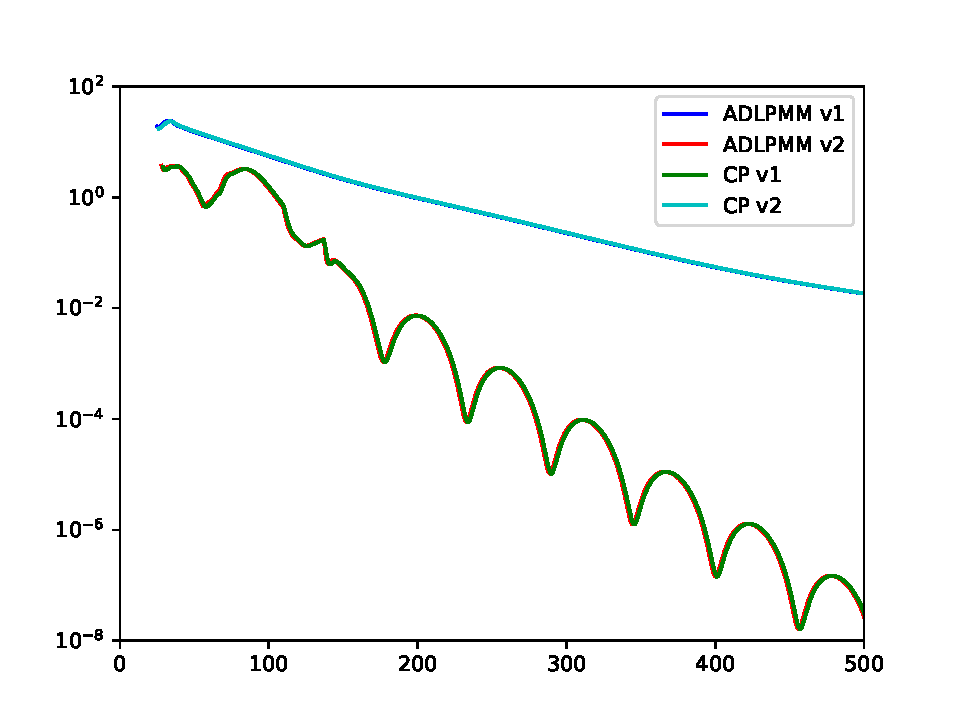
\includegraphics[width=14cm]{images/part3_ex2_fig1.pdf}
    \caption{$F(\bs x^k)-F_{\text{opt}}$ in log-scale along the 
  y-axis for the first 500 iterations of each of the methods 
  with all-zeros vectors and a constant stepsize. The optimal solution has been computed as the best one across 10000 iterations. }
  \label{fig:ex4}
\end{figure}

\indent (d) We consider now the problem
\begin{align*}
	\min \frac{\|\bs x \|^2_2}{2} + \left\{-\sum_{i=1}^m\log\left(\bs a_i^\top \bs x - b_i\right)+ \sum_{i=1}^{n-2} \sqrt{\left(x_i-x_{i+1}\right)^2+\left(x_{i+1}-x_{i+2}\right)^2}: a_i^\top \bs x > b_i, i\in [m] \right\}. 
\end{align*}
This fits the CP framework with $f = h_2$ and $g(\bs x)=\frac{\|\bs x \|^2_2}{2}$ which is $1$-strongly convex, and has a proximal operator given by
\begin{align*}
	\text{prox}_{\frac{\lambda\|\bs x \|^2_2}{2}}(\bs x) = \frac{\bs x}{\lambda+1}. 
\end{align*}
This leads to the following ACP method: 
  \begin{align*}
    \begin{split}
    \left\{
    \begin{array}{ll}
       \bs y^{k+1} &= \bs y^k + \sigma_k \bs A\left(\bs x^k + \theta_k \left( \bs x^{k}-\bs x^{k-1}\right)\right)- \sigma_k \text{prox}_{\tinv \sigma_k h_2}\left[\frac{\bs y^k + \sigma_k \bs A\left(\bs x^k + \theta_k \left( \bs x^{k}-\bs x^{k-1}\right)\right)}{\sigma_k} \right]\\
       \bs x^{k+1} &= \frac{\bs x^k - \tau_k\bs A^\top \bs y^{k+1}}{\tau_k+1}\\
       \theta_{k+1} &= \frac{1}{\sqrt{1+\tau_k}},\quad \tau_{k+1} = \theta_{k+1}\tau_k,\quad \sigma_{k+1} = \frac{\sigma_k}{\theta_{k+1}}.
    \end{array}
    \right.
    \end{split}
    \end{align*}
    
 The above problem also fits the FDPG canonical problem 
 \begin{align*}
 	\min \left\{ f(\bs x) + g(\bs{Ax})\right),
 \end{align*}
 with $f(\bs x)=\frac{\|\bs x \|^2_2}{2}$ which is $1$-strongly convex and $g(\bs x)=h_2(\bs x)$. We also obtain that
 \begin{align*}
	\underset{\bs u}{\text{argmax}} \left\{\left \langle \bs u, \bs A^\top \bs y \right \rangle - f(\bs u)\right\} &= \underset{\bs u}{\text{argmax}} \left\{\left \langle \bs u, \bs A^\top \bs y \right \rangle - \tinv 2\norm{\bs u}{2}^2 \right\} = \bs A^\top \bs y. 
\end{align*}
This leads to the following FDPG method:
     \begin{align*}
    \begin{split}
    \left\{
    \begin{array}{ll}
         \bs u^{k} &= \bs A^\top \bs w^k\\
        \bs y^{k+1} &= \bs w^k-\tinv L \bs{Au}^k + \tinv L \text{prox}_{Lh_2}\left(\bs{Au}^k-L\bs w^k\right) \\
        t_{k+1} &= \frac{1+\sqrt{1+4t_k^2}}{2} \\
        \bs w^{k+1} &= \bs y^{k+1} + \left( 
        \frac{t_k-1}{t_{k+1}} \right) (\bs y^{k+1}- \bs y^k)
    \end{array}
    \right.
    \end{split}
    \end{align*}
    and with  $\bs x^k = \bs A^\top \bs y^k$.
    
\indent (e) Both methods have been implemented.  The results are presented on \Cref{fig:ex42} with more iterations than what is written in the statement as otherwise most of the iterations are not feasible. We observe that the ACP method works way better than the FDPg one. More precisely, the first three components of the obtained solution (after $100$ iterations) are given by
           \begin{align*}
       \bs x^{*,\text{ACP}} &= [ 1.160,  1.986, -1.285,\hdots],\\
        \bs x^{*,\text{FDPG}} &= [1.140,  1.945, -1.245,\hdots].
       \end{align*}
    \begin{figure}[H]
    \centering
    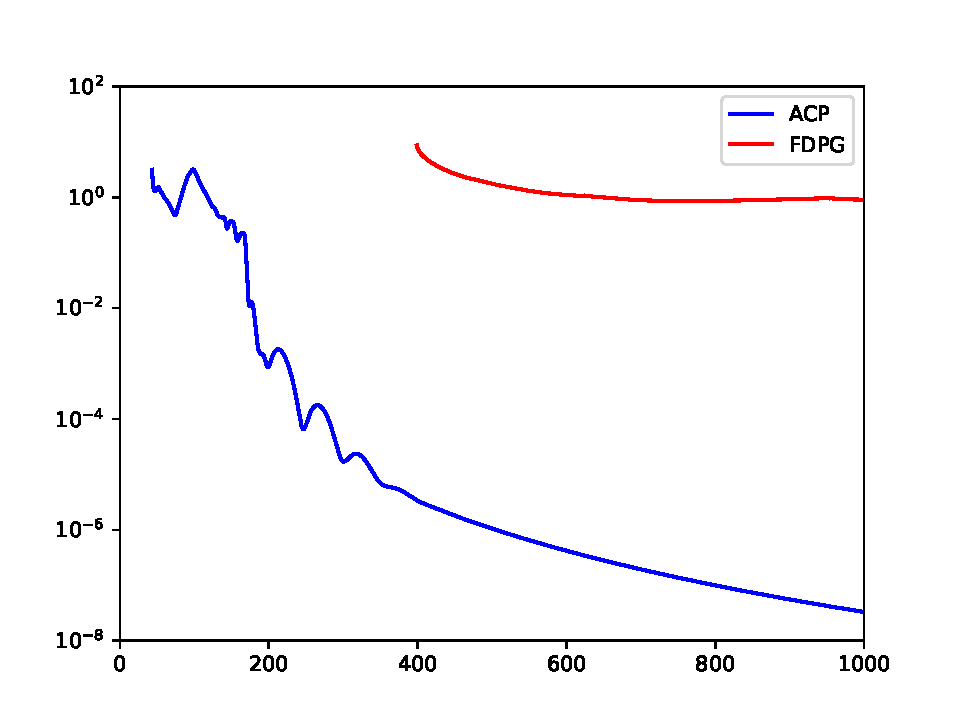
\includegraphics[width=14cm]{images/part3_ex2_fig2.pdf}
    \caption{$F(\bs x^k)-F_{\text{opt}}$ in log-scale along the 
  y-axis for the first 1000 iterations of each of the methods 
  with all-zeros vectors and a constant stepsize. The optimal solution has been computed as the best one across 10000 iterations. }
  \label{fig:ex5}
\end{figure}
On the above figure, FDPG does not seem to converge. Yet, looking at more iterations, we obtain the following result, on which we indeed see FDPG converges. 
    \begin{figure}[H]
    \centering
    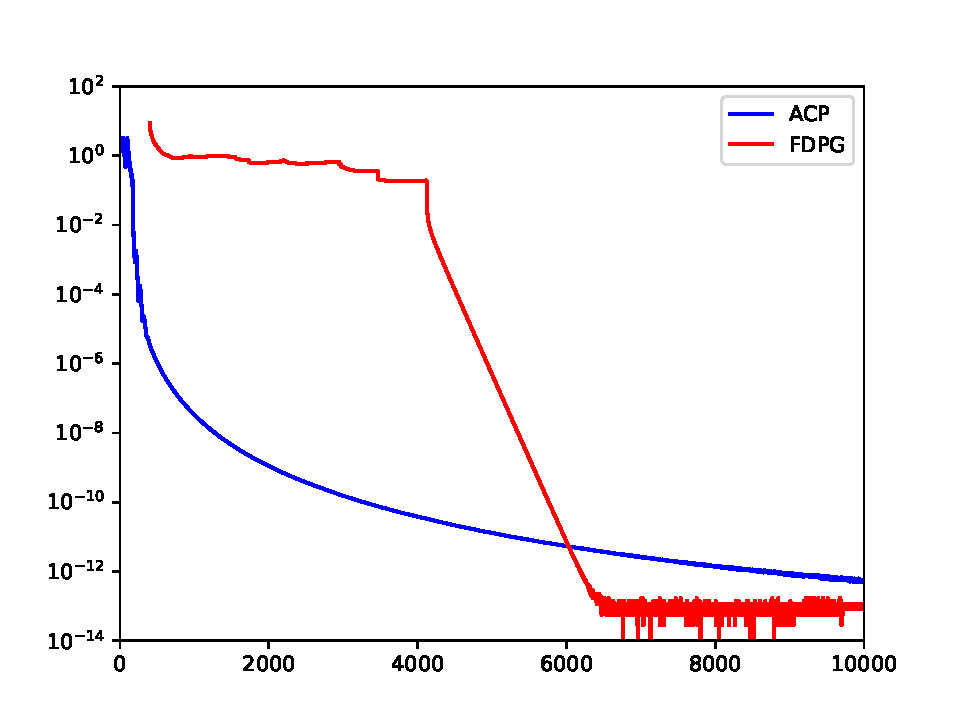
\includegraphics[width=14cm]{images/part3_ex2_fig3.pdf}
    \caption{$F(\bs x^k)-F_{\text{opt}}$ in log-scale along the 
  y-axis for the first 10000 iterations of each of the methods 
  with all-zeros vectors and a constant stepsize. The optimal solution has been computed as the best one across 10000 iterations. }
  \label{fig:ex6}
\end{figure}